\chapter{Конструкторская часть}

В данном разделе предсатвлены требования к программному обеспечению, а также схемы алгоритмов, выбранных для решения поставленной
задачи.

\section{Требования к программному обеспечению}
Программа должна предоставлять доступ к функционалу:
\begin{itemize}
	\item задать направление взгляда камеры;
	\item изменение положения источника света;
	\item конфигурация облачного неба с помощью загрузки погодной карты;
	\item варьирование параметров облачного неба;
\end{itemize}

К программе предъявляются следующие требования:
\begin{itemize}
	\item время отклика программы должно быть менее 50 мс;
	\item программа должна корректно реагировать на любые действия пользователя;
\end{itemize}

\section{Разработка алгоритмов}

Алгоритм Ray Marching применяется для визуализации облачного неба. 

Для повышения эффективности алгоритма Ray Marching необходимо снизить количество шагов вне облака. Для этого применяются объемлющие оболочки, в данном случае, такими оболочками будут являться сферы. Когда луч пересекает оболочку, необходимо сделать $ N $ шагов, на каждом из которых вычисляется плотность в точке пространства и ее освещенность, используя эти данные итеративно вычисляется значение цвета пикселя. 

Как показано на рисунке \ref{fig:earth}, атмосфера будет моделироваться с помощью двух концентрических сфер, между которыми и будет происходить генерация облаков.

\begin{figure}[h]
	\centering
	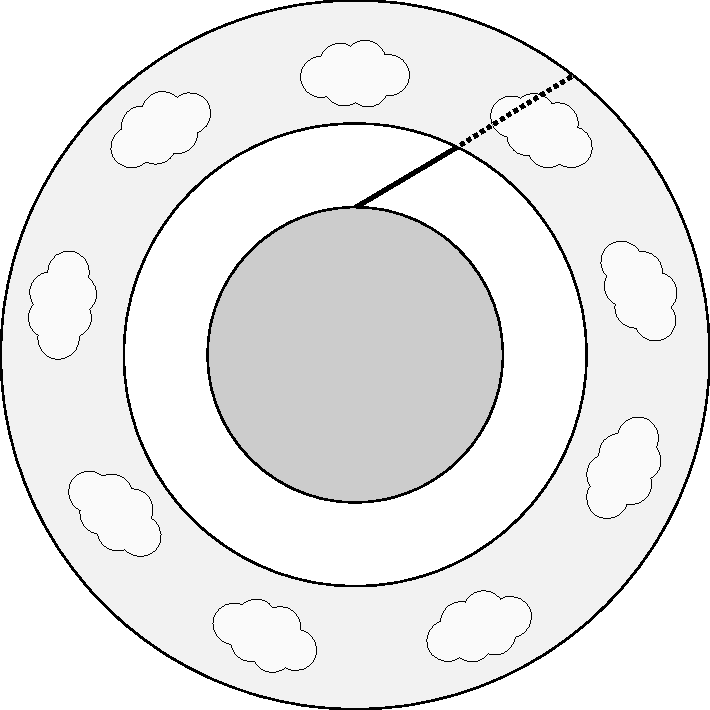
\includegraphics[width=0.8\textwidth]{assets/img/earth.pdf} % замените на имя вашего файла
	\caption{Схема атмосферы и положения наблюдателя}
	\label{fig:earth}
\end{figure}

\subsection{Пересечение луча со сферой}

Уравнение луча запишем следующим образом:

\begin{equation}
	\label{ray_eq}
	P = S + t \vec{D}, t \ge 0
\end{equation}
где $ S $ - точка, откуда луч испускается, а $ \vec{D} $ - направление луча.

Пусть сфера задается своим центром $ C $ и радиусом $ r $. Если луч пересекает сферу, тогда точка $ P $ - лежит на поверхности, запишем это следующим образом:

\begin{equation}
	\label{ray_intersec_sp}
	\| P - C \| = r
\end{equation}

Перепишем \eqref{ray_intersec_sp}, используя скалярное произведение:
\begin{equation}
	\label{ray_intersec_sp2}
	\sqrt{\langle P - C , P - C \rangle} = r
\end{equation}

Подставим в \eqref{ray_intersec_sp2} уравнение луча \eqref{ray_eq}:

\begin{equation}
	\label{ray_intersec_sp3}
	\sqrt{\langle S + t \vec{D} - C , S + t \vec{D} - C \rangle} = r
\end{equation}

Обозначим $ S - C = \vec{SC} $ и раскроем скалярное произведение, возведя обе части уравнения \eqref{ray_intersec_sp3} в квадрат:

\begin{equation}
	\label{ray_intersec_sp4}
	t ^ 2 \langle \vec{D}, \vec{D} \rangle + 2t \langle \vec{SC}, \vec{D} \rangle + \langle \vec{SC}, \vec{SC} \rangle - r ^ 2 = 0
\end{equation}

Решая квадратное уравнение \eqref{ray_intersec_sp4} находим точки пересечения луча с объемлющей оболочкой.

\subsection{Вычисление плотности облаков в атмосфере}

Как было описано в пункте \ref{implicit}, для представления поля плотности облаков будем хранить две объемные текстуры.
Первая (основная) текстура отвечает за низкочастотный шум, имеет размер $ 128 \times 128 \times 128 $. Вторая (вспомогательная) текстура отвечает за высокочастотный шум, имеет размер $ 32 \times 32 \times 32 $. 
В таблице \ref{tab:textures} показаны какие шумы используются для формирования текстур.

\begin{table}[b]
	\begin{center}
\begin{tabular}{|c|c|c|c|c|}
	\hline
	Текстура & \multicolumn{4}{c|}{Шумы} \\
	\hline
	Основная & П-В (НЧ) & В (НЧ) & В (СЧ) & В (ВЧ)\\
	\hline
	Вспомогательная & В (НЧ) & В (СЧ) & В (ВЧ) & -\\
	\hline
\end{tabular}
\end{center}
\caption{Таблица шумов, из которых состоят текстуры. П-В - шум Перлина-Ворлея, В - шум Ворлея, НЧ - низкая частота, СЧ - средняя частота, ВЧ - высокая частота}
\label{tab:textures}
\end{table}

В итоге, чтобы рассчитать плотность в некоторой точке, необходимо получить срезы шумов из текстуры и составить из них fBM (англ. fractal Brownian motion). FBM представляет собой сумму ряда октав шума, каждая из которых имеет более высокую частоту и более низкую амплитуду.

Основная текстура применяется для формирования общей грубой формы облака и может использоваться для определения факта попадания луча в облако. Вспомогательная текстура используется для добавления деталей на поверхности облака.

Для возможности формировать облачное небо используются погодные карты. Погодная карта является двумерной текстурой, и состоит из трех каналов RGB, где в R канале хранится процент покрытия неба облаками, G хранит тип облаков, B канал может быть использован для хранения вероятности возникновения дождя, но в данном алгоритме он не будет использоваться. 

Тип облаков будем задавать с помощью функции, которая рассеивает облако в зависимости от его высоты. 

В итоге плотность в данной точке вычисляется с помощью базовой плотности, полученной из текстуры, затухания, полученного из функции типа облака и R канала погодной карты. 

\subsection{Общий алгоритм построения изображения}

Общий алгоритм построения изображения показан на рисунке \ref{fig:renderscheme}.

\begin{figure}
	\centering
	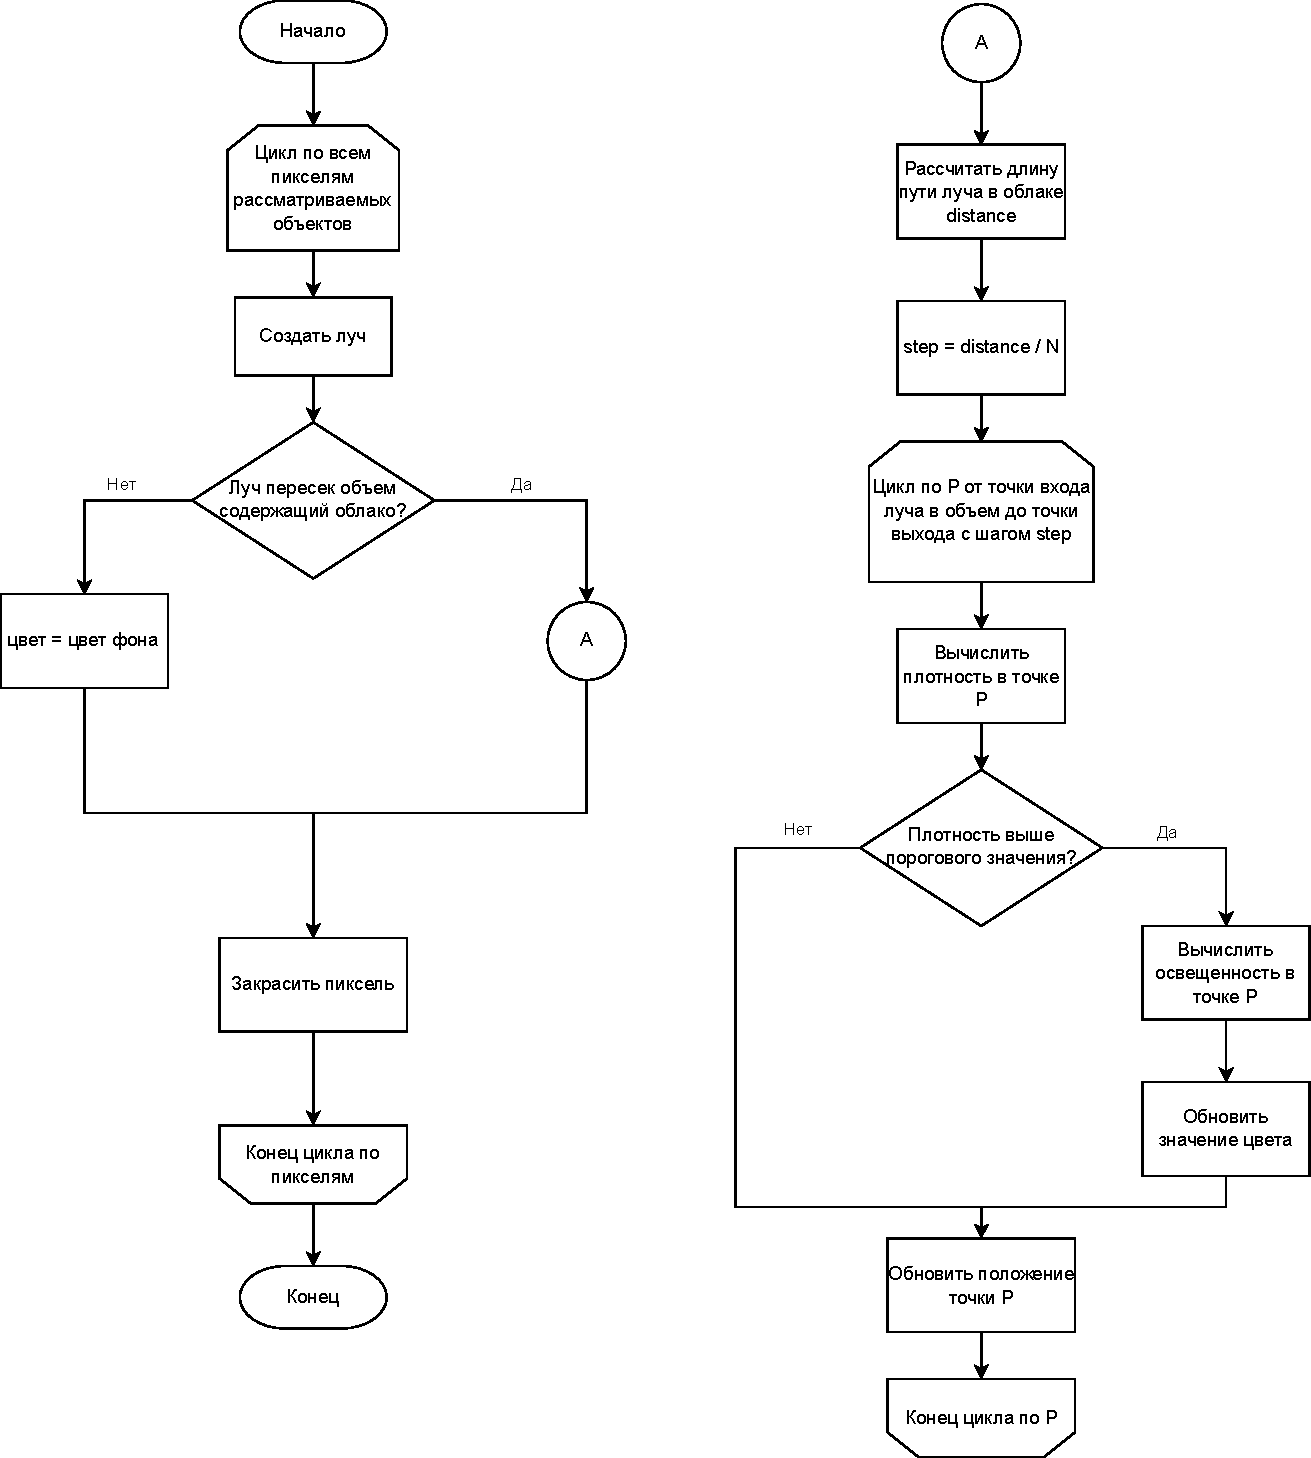
\includegraphics[width=1\textwidth]{assets/img/renderscheme2.pdf} % замените на имя вашего файла
	\caption{Схема визуализации облаков с помощью алгоритма Ray Marching}
	\label{fig:renderscheme}
\end{figure}

\newpage

\section{Выбор используемых типов и структур данных}

В данной работе используются следующие типы и структуры данных:
\begin{enumerate}
	\item источник света -- задается направлением и интенсивностью;
	\item облака -- задаются с помощью объемных текстур, погодной карты, функций рассеивания;
	\item текстура -- задается с помощью двумерных и трехмерных массивов, состоящих из цветов;
	\item цвет -- хранит три или четыре составляющие RGB или RGBA модели цвета соответственно;
	\item математические абстракции: 
		\begin{itemize}
			\item точка -- хранит координаты x, y, z;
			\item вектор -- хранит направление по x, y, z;
		\end{itemize}
\end{enumerate}


\section*{Вывод}
В данном разделе были представлены требования к разрабатываемому
программному обеспечению и разработана схема разрабатываемого алгоритма.
Так же, были описаны структуры данных, которые будут использоваться при реализации программного обеспечения.

